
\chapter{Movimiento del cuerpo rígido}

\section{Movimiento Circular Uniforme}

Considere el movimiento descrito por la siguiente ecuaci\'on
\begin{align}
  \label{eq:mua}
  \mathbf{r}(t)=r\left(\hat{\mathbf{i}}\cos(\omega t)+\hat{\mathbf{j}}\sin(\omega t)\right),
\end{align}
con $r=\text{constante}$ y $\omega=\text{constante}$, representado en la figura~\ref{fig:mua1}.

La velocidad es
\begin{align}
  \mathbf{v}=&%detalles\\
  r\omega\left(-\hat{\mathbf{i}}\sin(\omega t)+\hat{\mathbf{j}}\cos(\omega t)\right),
\end{align}
representado en la figura~\ref{fig:mua2}. Note que $\mathbf{r}\cdot\mathbf{v}=0$, de modo que los vectores son perpendiculares.

La aceleraci\'on es
\begin{align}
  \mathbf{a}=&%detalles\\
  -r\omega^2\left(\hat{\mathbf{i}}\cos(\omega t)+\hat{\mathbf{j}}\sin(\omega t)\right),
\end{align}
representado en la figura~\ref{fig:mua3}. Note que $\mathbf{a}\cdot\mathbf{v}=0$, de modo que los vectores son perpendiculares. Adem\'as
$\mathbf{r}\cdot\mathbf{a}=-1$, de modo que los vectores son antiparalelos.


\begin{frame}[fragile,allowframebreaks]
  \begin{figure}
    \centering
    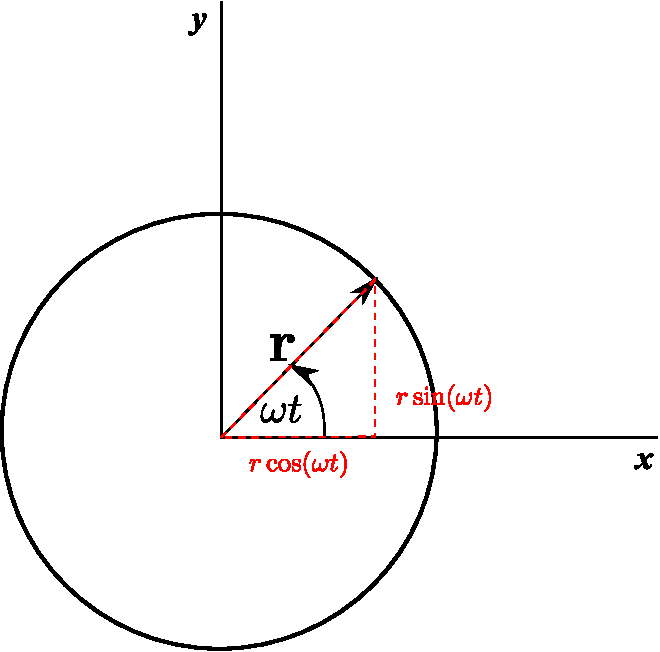
\includegraphics[scale=0.65]{mua1}    
    \caption{Posici\'on}
    \label{fig:mua1}
  \end{figure}

\end{frame}
\begin{frame}[fragile,allowframebreaks]
  \begin{figure}
    \centering
    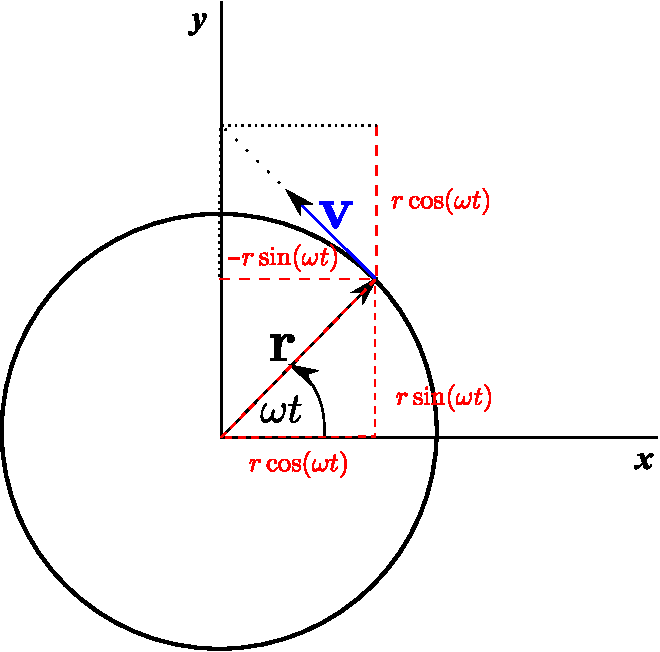
\includegraphics[scale=0.65]{mua2}    
    \caption{Velocidad: tangente a la curva}
    \label{fig:mua2}
  \end{figure}
\end{frame}

\begin{frame}[fragile,allowframebreaks]
  \begin{figure}
    \centering
    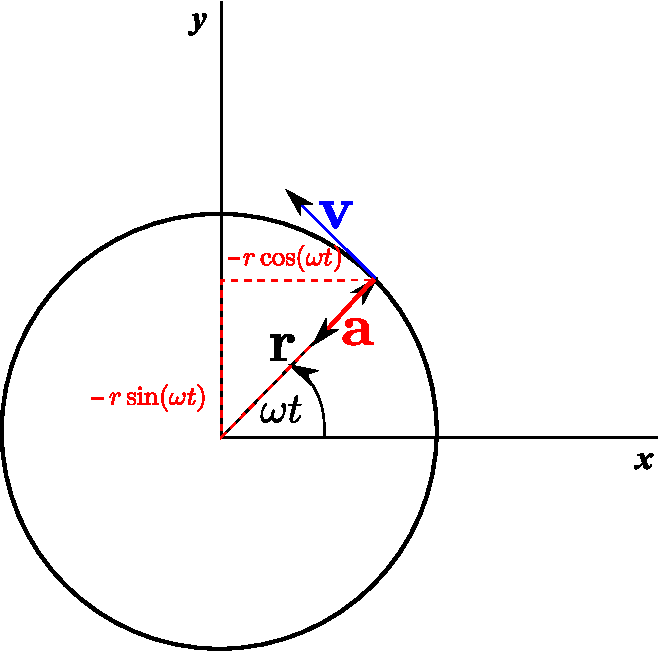
\includegraphics[scale=0.65]{mua3}
    \caption{Aceleraci\'on: centr\'\i peta}
    \label{fig:mua3}
  \end{figure}


\end{frame}

\subsection{Movimiento generalizado en coordenadas polares}

%Hacer una figura con los ejes rotados con hat theta a pi/2+theta 

La ecuaci\'on para el vector de posici\'on puede escribirse en general como
\begin{align}
\label{eq:rpol}
  \mathbf{r}(t)=&r(t)\left(\hat{\mathbf{i}}\cos[\theta(t)]+\hat{\mathbf{j}}\sin[\theta(t)]\right)\nonumber\\
=&r(t)\hat{\mathbf{r}}(t)
\end{align}
Para algunos problemas es conveniente reescribir \'esta ecuaci\'on en coordenadas polares, donde
\begin{align}
\label{eq:runit}
  \hat{\mathbf{r}}(t)=\hat{\mathbf{i}}\cos[\theta(t)]+\hat{\mathbf{j}}\sin[\theta(t)]\,.
\end{align}


El vector perpendicular a $\hat{\mathbf{r}}(t)$ describe la dirección angular. De la figura %ver notas
\begin{align}
\label{eq:thetaunit}
  \hat{\boldsymbol{\theta}}(t)=&\hat{\mathbf{i}}\cos[\pi/2-\theta(t)]+\hat{\mathbf{j}}\sin[\pi/2-\theta(t)]\nonumber\\
=&-\hat{\mathbf{i}}\sin[\theta(t)]+\hat{\mathbf{j}}\cos[\theta(t)]\,.
\end{align}

Las ecuaciones \eqref{eq:runit} y \eqref{eq:thetaunit} pueden escribirse en forma matricial


\begin{align}
  \label{eq:polinv}
  \begin{pmatrix}
    \hat{\mathbf{r}}\\
    \hat{\boldsymbol{\theta}}
  \end{pmatrix}=
  \begin{pmatrix}
    \cos\theta&\sin\theta\\
    -\sin\theta&\cos\theta\\
  \end{pmatrix}
  \begin{pmatrix}
    \;\hat{\mathbf{i}}\;\\
    \hat{\mathbf{j}}\\
  \end{pmatrix}.
\end{align}
con inverso
\begin{align}
  \begin{pmatrix}
    \;\hat{\mathbf{i}}\;\\
    \hat{\mathbf{j}}\\
  \end{pmatrix}=
  \begin{pmatrix}
    \cos\theta&-\sin\theta\\
    \sin\theta&\cos\theta\\
  \end{pmatrix}
  \begin{pmatrix}
    \hat{\mathbf{r}}\\
    \hat{\boldsymbol{\theta}}
  \end{pmatrix}.
\end{align}

De la ec.~\eqref{eq:rpol}, la velocidad es
\begin{align}
  \label{eq:vcurvprev}
  \mathbf{v}(t)=\dot{\mathbf{r}}(t)=\dot{r}(t)\hat{\mathbf{r}}(t)+
r(t)\dot{\hat{\mathbf{r}}}(t)\,.
\end{align}
Ahora, de la ec.~\eqref{eq:runit}
\begin{align}
  \dot{\hat{\mathbf{r}}}(t)=&\frac{d}{dt}\left(\hat{\mathbf{i}}\cos[\theta(t)]+\hat{\mathbf{j}}\sin[\theta(t)]\right)\nonumber\\
  =&\dot{\theta}
  \left(
    -\hat{\mathbf{i}}\sin[\theta(t)]+\hat{\mathbf{j}}\cos[\theta(t)]
  \right)
\end{align}
y usando la ec.~\eqref{eq:thetaunit}
\begin{align}
\dot{\hat{\mathbf{r}}}(t)=\dot{\theta}\hat{\boldsymbol{\theta}}\,.
\end{align}
Sustituyendo en la ec.~\eqref{eq:vcurvprev}:
\begin{align}
  \label{eq:vpol}
  \mathbf{v}(t)=&\dot{r}(t)\hat{\mathbf{r}}(t)+r(t)\dot{\theta}(t)\hat{\boldsymbol{\theta}}(t)\nonumber\\
  =&\dot{r}(t)\hat{\mathbf{r}}(t)+r(t)\omega(t)\boldsymbol{\theta}(t)\,.
\end{align}
donde hemos definido la velocidad angular instantánea como
\begin{align}
  \omega(t)=\dot\theta(t)
\end{align}

y la aceleraci\'on es %ver notas
\begin{align}
\label{eq:apol}
  \mathbf{a}(t)=&%detalles\\
[\underbrace{\ddot{r}(t)}_{{\text{Acel. lineal.}}}
-\underbrace{r(t)\dot{\theta}^2(t)}_{{\text{Acel. centr\'\i peta.}}}]\hat{\mathbf{r}}(t)
+[\underbrace{r(t)\ddot{\theta}(t)}_{{\text{Acel. lineal tangencial.}}}
+\underbrace{2\dot{r}(t)\dot{\theta}(t)}_{{\text{Acel. de coriolis.}}}]\hat{\boldsymbol{\theta}}(t).
\end{align}

\ejemplo{\textbf{MCU}:}
Calcule la fuerza para mantener un cuerpo de masa $m$ en un movimiento circular uniforme


Comparando (\ref{eq:mua}) con (\ref{eq:rpol}), tenemos para el Movimiento Circular Uniforme que
\begin{align}
  \label{eq:muapol}
   \dot{r}=&0&&&&\\
  \theta(t)=&\omega t\,,&\dot{\theta}(t)=&\omega\,,&\ddot{\theta}(t)=&0\,.
\end{align}
De modo que reemplazando las ecuaciones \eqref{eq:muapol} en las ecuaciones \eqref{eq:vpol}, \eqref{eq:apol}, y usando la transformaci\'on inversa \eqref{eq:polinv}, tenemos que
\begin{align}
  \mathbf{r}(t)=&r\hat{\mathbf{r}}(t)\nonumber\\
  =&r\left(\hat{\mathbf{i}}\cos(\omega t)+\hat{\mathbf{j}}\sin(\omega t)\right),
\end{align}
\begin{align}
    \mathbf{v}(t)=&r\omega\hat{\boldsymbol{\theta}}(t)\nonumber\\
    =&r\omega\left(-\hat{\mathbf{i}}\sin(\omega t)+\hat{\mathbf{j}}\cos(\omega t)\right),
\end{align}
en magnitud:
\begin{align}
  \label{eq:vome}
  v=r\omega\,.
\end{align}

La siguiente derivada da lugar a 
\begin{align*}
  \mathbf{a}(t)=\dot{\mathbf{v}}(t)=&-r(t)\omega^2(t)\hat{\mathbf{r}}(t)\nonumber\\
  =&-\frac{(r\omega)^2}{r}\hat{\mathbf{r}}\,,
\end{align*}
y usando la ec.\eqref{eq:vome}
\begin{align}
  \mathbf{a}(t)=-\frac{v^2}{r}\hat{\mathbf{r}}
\end{align}

de modo que en el MCU la velocidad no tiene componente radial, y s\'olo
contribuye la aceleraci\'on centr\'\i peta, como era de esperarse. Finalmente
\begin{align}
  \mathbf{F}=m\mathbf{a}=-\frac{m v^2}{r}\hat{\mathbf{r}}\,.
\end{align}


\qed

%theta es theta_z y la direccion de omega_z es a lo largo del eje z


\ejemplo{} 
\label{eje:movim-gener-en}
Calcular la velocidad de rotación de una partícula de masa
girando en movimiento circular en una plano paralelo al plano $x$-$y$
y con el eje $z$ pasando por el centro de la orbita circular.

%hacer dibujo obtener la formula para la velocidad en términos de la
%velocidad angular.  ver notas en estrellitas

\begin{align*}
  \mathbf{v}=\boldsymbol{\omega}\times\mathbf{r}\,.
\end{align*}

\qed


Las componentes angulares como tal:
\begin{align*}
  \theta_x\hat{\mathbf{i}}+\theta_y\hat{\mathbf{j}}+\theta_k\hat{\mathbf{k}}\,,
\end{align*}
no pueden formar un vector, pues no resultaria ser conmutativo, como
puede mostrarse facilmente haciendo rotaciones sobre los tres ejes de
un libro en el espacio. La diferencia entre las diferentes
posibilidades de rotaciones son del orden de $\Delta
\theta_{x,y,x}^2$, de modo que las componentes diferenciales si forman
un vector. 

Definimos entonces la velocidad angular en tres dimensiones como:
\begin{align}
  \boldsymbol{\omega}=&\frac{d\theta_x}{dt}\hat{\mathbf{i}}+\frac{d\theta_y}{dt}\hat{\mathbf{j}}
+\frac{d\theta_z}{dt}\hat{\mathbf{k}}\nonumber\\
=&\omega_x\hat{\mathbf{i}}+\omega_y\hat{\mathbf{j}}+\omega_z\hat{\mathbf{k}}\,.
\end{align}
La ecuacion obtenida en el ejemplo~\ref{eje:movim-gener-en} es válida
en general
\begin{align}
  \mathbf{v}=\boldsymbol{\omega}\times\mathbf{r}\,.
\end{align}

%\left(\right)

\section{Momentum angular y torque para una partícula}
Definimos el momento angular para una partícula de moméntum $\mathbf{p}$ como
\begin{align}
  \label{eq:L}
  \mathbf{L}=&\mathbf{r}\times\mathbf{p}\,.
\end{align}
y el correspondiente vector de torque como el causante de los cambios
en el momento angular cuando son aplicados durante algún intervalo
$\Delta t$ sobre la partícula.
\begin{align}
  \Delta \mathbf{L}\approx \boldsymbol{\tau}\Delta t\,.
\end{align}
Entonces
\begin{align}
  \boldsymbol{\tau}=\frac{d\,\mathbf{L}}{dt}\,.
\end{align}
Desarrollando esta expresión, tenemos que
\begin{align}
  \boldsymbol{\tau}=&\frac{d}{dt}\left(\mathbf{r}\times\mathbf{p}\right)\nonumber\\
=&\left(\frac{d\mathbf{r}}{dt}\right)\times\mathbf{p}+
\mathbf{r}\times\frac{d\mathbf{p}}{dt}\nonumber\\
=&\mathbf{v}\times\mathbf{p}+
\mathbf{r}\times\frac{d\mathbf{p}}{dt}\nonumber\\
\end{align}
como $\mathbf{v}$ es paralelo a $\mathbf{p}$, la variación del
momentum es la fuerza aplicada, entonces
\begin{align}
  \label{eq:torque}
  \boldsymbol{\tau}=\mathbf{r}\times\mathbf{F}\,.
\end{align}

Para entender las definiciones de moméntum angular y torque es mejor
ir hacia atras del resultado en \eqref{eq:torque} la resultado en
\eqref{eq:L}: La capacidad de una fuerza para ejercer un giro sobre
una partícula depende de la distancia a la que es aplicada la fuerza.
%\left(\right)

\section{Momentum angular para un cuerpo rígido}


El moméntum angular para un cuerpo rígido es la suma del momentum
angular para cada partícula en el cuerpo rígido como se ilustra en la
fig.~\ref{fig:centrodemasarigido}

\begin{frame}
\begin{figure}
  \centering
  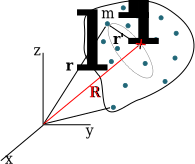
\includegraphics{centrodemasarigido}
  \caption{Cuerpo rígido}
  \label{fig:centrodemasarigido}
\end{figure}
\end{frame}
\begin{align}
  \mathbf{L}=\sum_{i=1}^N\mathbf{L}_i=\sum_{i=1}^N \mathbf{r}_i\times m_i\dot{\mathbf{r}}_i
\end{align}
Usando la relación entre las coordenas con respecto a una sistema
externo y las coordenadas del centro de masa
\begin{align}
  \mathbf{r}_i=\mathbf{R}+\mathbf{r}_i'\,,
\end{align}

\begin{align}
   \mathbf{L}=&\sum_{i=1}^N
   \left(\mathbf{R}+\mathbf{r}_i'\right)\times m_i
   \left(\dot{\mathbf{R}}+\dot{\mathbf{r}}_i'\right)
\end{align}
Analicemos término a término
\begin{align*}
  \sum_{i=1}^N\mathbf{R}\times m_i\dot{\mathbf{R}}
\end{align*}

Que puede escribirse en el sistema de centro de masa, $\mathbf{r}_i'$, como % detalles en notas del cuaderno
\begin{align}
  \label{eq:lcm}
   \mathbf{L}=\mathbf{R}\times M\mathbf{V}+\sum_{i=1}^N \mathbf{r}_i'\times m_i\dot{\mathbf{r}}_i'\,,
\end{align}

\begin{align}
  \label{eq:tensorI}
  \mathbf{L}=\mathbf{R}\times M\mathbf{V}+\mathbb{I}\boldsymbol{\omega}\,,
\end{align}
y el moméntum angular alrededor del centro de masa es
\begin{align}
  \mathbf{L}_0=\mathbb{I}\boldsymbol{\omega}\,.
\end{align}

El moméntum angular puede entonces dividirse en dos partes
\begin{itemize}
\item $\mathbf{L}_{\text{trans}}$: Momento angular debido a la rotación del cuerpo sobre su centro de masa
\item $\mathbf{L}_{\text{rot}}$: Momento angular debido al movimiento del centro de masa con respecto al origen del sistema inercial de coordenadas.
\end{itemize}

\section{Torque}

Definimos el torque sobre un cuerpo rígido como la derivada temporal de su moméntum angular:
\begin{align}
  \label{eq:torque}
  \boldsymbol{\tau}=\frac{d\mathbf{L}}{dt}\,.
\end{align}
Esta ecuación define el \emph{Principio de Moméntum Angular}. 

Tomando la derivada temporal en la ec.~(\ref{eq:lcm}), y usando
\begin{align}
  \mathbf{F}=\sum_{i=1}^N\mathbf{f}_i\,,
\end{align}
tenemos
\begin{align}
  \boldsymbol{\tau}=&\sum_{i=1}^N\mathbf{r}_i'\times \mathbf{f}_i+\mathbf{R}\times\mathbf{F}\,,
\end{align}
El primer termino corresponde al torque sobre el centro de masa debido a las diversas fuerzas externas, y el segundo término es el torque debido a la fuerza externa total actuando sobre el centro de masa

Similarmente, tomando la derivada de la expresión para el moméntum en la ec.~(\ref{eq:tensorI})
\begin{align}
  \boldsymbol{\tau}=&\mathbb{I}\frac{d\boldsymbol{\omega}}{dt}+\mathbf{R}\times M\frac{\mathbf{V}}{dt}\nonumber\\
=&\mathbb{I}\boldsymbol{\alpha}+\mathbf{R}\times M\mathbf{a}\,.
\end{align}


En el caso de una partícula, si una fuerza ejerce un torque relativo a una localización $A$
\begin{align}
  \boldsymbol{\tau}_A=\mathbf{r}_A\times\mathbf{F}
\end{align}
dicho torque causa cambios en el moméntum angular dados por el principio de moméntum angular
\begin{align}
  \frac{d\mathbf{L}}{dt}=&\boldsymbol{\tau}_A&\text{ó}\qquad \Delta\mathbf{L}\approx& \boldsymbol{\tau}_A \Delta t\,.
\end{align}



\subsection{Conservación del moméntum angular}
Como los torques de los pares de fuerzas de acción reacción son iguales y opuestos, entonces al torque neto sobre un sistema de partículas sólo contribuyen las fuerzas externas

La ec.~(\ref{eq:torque}) la podemos escribir más explícitamente como
\begin{align}
  \label{eq:torqueneto}
  \boldsymbol{\tau}_{\text{neto}}=\frac{d\mathbf{L}}{dt}\,.
\end{align}
Podemos observar que si el torque neto alrededor de una localización
$A$ es cero, el moméntum angular sobre esa localización no cambia.

Pueden existir fuerzas actuando, causando cambios en el moméntum
lineal, pero si las fuerzas no ejercen ningún torque, la tasa de
cambio del moméntum angular es cero y se conserva. Por ejemplo en el
caso de la interacción de dos cuerpos que se mueven bajo el efecto de
una fuerza con sólo componente radial, la cual no ejerce torques,
entonces el moméntum angular del sistema se debe conservar. Este es el
caso de las orbitas planetarias.


\section{Energía cinética rotacional}
Expresando la energía cinética de un cuerpo rígido 
\begin{align}
  K\frac{1}{2}\sum_{i=1}^N m_i v_i^2\,,
\end{align}
en la coordenadas del centro de masa, tenemos
\begin{align}
  K=&\frac{1}{2}M V^2+\frac{1}{2}\boldsymbol{\omega}\cdot
  \mathbf{L}_0\nonumber\\
0&\frac{1}{2}M V^2+\frac{1}{2}\boldsymbol{\omega}\cdot
  \left(\mathbb{I}\boldsymbol{\omega}\right)\,.
\end{align}
Cuando $\mathbf{L}_0$ y $\boldsymbol{\omega}$ están referidos a los ejes principales de inercia
\begin{align}
  K=\frac{1}{2}MV^2+\frac{1}{2}I_1\omega_1^2+\frac{1}{2}I_2\omega_2^2+\frac{1}{2}I_3\omega_3^2\,.
\end{align}

\section{Teorema de los ejes paralélos}

Sea $I_0$ el momento de inercia sobre un eje pasando por el centro de masa de un cuerpo de masa $M$. El momento de inercia sobre un eje paralelo a $I_0$ es
\begin{align}
  I=I_0+M l^2\,,
\end{align}
donde $l$ es la distancia entre los ejes.

\begin{itemize}
\item[\textbf{Demostación}] La ecuación que relaciona las coordenadas en el sistema de centro de masa para una partícula del cuerpo rígido es
  \begin{align}
    \mathbf{r}_i=&\mathbf{R}+\mathbf{r}'_i\nonumber\\
    (x_i,y_i,z_i)=&(x'_i,y'_i,z'_i)+(R_x,R_y,R_z)\nonumber\\
    \boldsymbol{\rho}_i+z_i\hat{\mathbf{k}}=& \mathbf{R}_T+R_z\hat{\mathbf{k}}+\boldsymbol{\rho}'_i+z'_i\hat{\mathbf{k}}\,.
  \end{align}
Igualando las componentes transversales tenemos
\begin{align}
  \boldsymbol{\rho}_i=& \mathbf{R}_T+\boldsymbol{\rho}'_i
\end{align}
Elevando al cuadrado y sumando sobre todas las masas tenemos el momento de inercia alrededor de un eje paralelo al del centro de masa que fijamos para que coincida con el eje $z$
\begin{align}
  I=\sum_i m_i\boldsymbol{\rho}_i^2=&\sum_i m_i(\mathbf{R}_T+\boldsymbol{\rho}'_i)^2\,,
\end{align}
el producto cruzado de nuevo es cero por la definición de centro de masa
\begin{align}
  I=\sum_i m_i\boldsymbol{\rho}_i^2=&\sum_i m_i\mathbf{R}_T^2+\sum_i m_i{\boldsymbol{\rho}'}_i^2\nonumber\\
  =&M\mathbf{R}_T^2+\sum_i m_i{\boldsymbol{\rho}'}_i^2\,.
\end{align}
El momento de inercia alrededor del centro de masa es
\begin{align}
  I_0=\sum_i m_i{\boldsymbol{\rho}'}_i^2\,,
\end{align}
y $l=\left|\mathbf{R}_T\right|$ es la distancia entre los ejes de modo que
\begin{align}
  I=I_0+M l^2\,,
\end{align}
\end{itemize}


\section{Resumen}
\begin{enumerate}
\item Rotación pura sobre un eje sin traslación
  \begin{align}
    L=&I\omega\nonumber\\
    \tau=&I\alpha\nonumber\\
    K=&\tfrac{1}{2}I\omega^2\,.
  \end{align}
\item Rotación y traslación sobre un eje $z$ (el subíndice cero se refiere al centro de masa)
  \begin{align}
    L_z=&I_0\omega+(\mathbf{R}\times M\mathbf{V})_z\nonumber\\
    \tau_z=&\tau_0+(\mathbf{R}\times\mathbf{F})_z\nonumber\\
    \tau_0=&I_0\alpha\nonumber\\
    K=&\tfrac{1}{2}I_0\omega^2+\tfrac{1}{2}M V^2\,.
  \end{align}


\end{enumerate}


\section{Cálculo de moméntos de inercia}

\subsection{Varilla uniforme}

\subsection{Disco uniforme}
\subsection{Esfera}


\begin{itemize}
\item[\textbf{Ejemplo}]     Un cilíndro de radio $R$ y masa $M$ rueda sin deslizar a lo largo
    de una superficie debido a una cinta delgada enrollada en torno de
    el, que pasa por una polea ideal y está conectada a un bloque de
    masa $m$ como se muestra en la figura~\ref{fig:cilindropol}. Un estudiante obtiene la siguiente respuesta para la aceleración del cuerpo:
    \begin{align*}
      a_{\text{CM}}=\frac{4mg}{8m-3M}\,.
    \end{align*}
Justifique porqué dicha respuesta es incorrecta. 

\item[\textbf{Solución:}] El cilindro podría moverse hacia la izquierda.


\end{itemize}

\section{Problemas resueltos}

\begin{itemize}
\item[\textbf{Ejemplo}] Dos masas $m_1$ y $m_2$ unidas por una cuerda ideal están enrrolladas en una polea de radio $R$ y masa $M$ que puede rotar alrededor de un eje fijo que pasa por el centro de la polea, tal como se muestra en la figura~\ref{fig:polea}. Suponga que no hay fricción en el eje de la polea, que las dos masas están inicialmente en reposo, que $m_1 > m_2$ y que las dos masas están originalmente separadas una distancia $h$. Calcule la rapidez de cada una de las masas justamente cuando una pasa al lado de la otra, es decir, la rapidez de encuentro.

  \begin{figure}
    \centering
    \includegraphics[scale=0.8]{polea}
    \caption{Ejemplo conservación de la energía}
    \label{fig:polea}
  \end{figure}
La conservación de la energía mecánica se debe aplicar al sistema completo de masas $m_1$ y 
\end{itemize}



\begin{itemize}
\item[\textbf{Ejemplo:}] Tomado de \cite{mit2009}. Un péndulo físico consiste de una varilla uniforme de masa $m_1$ con un pivote en un extremo. La varilla tiene longitud $l_1$ y momento de inercia $I_1$  sobre le punto del pivote. Un disco de masa $m_2$ y radio $r_2$ con momento de inercia $I_{\text{cm}}$ sobre su centro de masa está unido rígidamente a una distancia $l_2$ del punto de pivote. El péndulo está inicialmente desplazado a un ángulo $\theta_0$ y entonces es liberado desde el reposo.
  \begin{enumerate}
  \item ¿Cual es el momento de inercia del péndulo físico sobre el punto de pivote?
    \label{item:1}
  \item ¿Cuan lejos del punto de pivote está el centro de masa del sistema?
    \label{item:2}
  \item ¿Cual es la velocidad angular del péndulo cuando el péndulo cuando el péndulo está en la parte de abajo de su oscilación?
\label{item:3}

\ref{item:1}. El momento de inercia sobre el punto de pivote será la suma del momento de inercia de la varilla, dada por $I_1$, y el momento de inercia del disco sobre el punto de pivote. El momento de inercia del disco sobre el punto de pivote se encuentra a partir del teorema de los ejes paralelos:
\begin{align}
  I_{\text{disc}}=I_{\text{cm}}+m_2 l_2^2\,.
\end{align}
El momento de inercia total sobre el punto de pivote es entonces
\begin{align}
  \label{eq:rig3}
  I_S=I_1+I_{\text{disc}}=I_1+I_{\text{cm}}+m_2 l_2^2\,.
\end{align}

\ref{item:2}. El centro de masa del sistema compuesto esta localizado a una distancia del punto de pivote dada por
\begin{align}
  \label{eq:rig5}
  l_{\text{cm}}=\frac{m_1(l_1/2)+m_2 l_2}{m_1+m_2}
\end{align}

\ref{item:3}. Podemos usar la conservación de la energía mecánica, para encontrar la velocidad angular del péndulo en la para de abajo de su oscilación. 

Tomando el punto de energía potencial gravitacional cero como el punto donde la parte de abajo de la varilla está en su posición más baja, esto es, $\theta=0$, tenemos que la energía mecánica inicial es (ver Figura~\ref{fig:pendulofisico})
\begin{align}
  E_0=U_0=m_1 g  \left(l_1-\frac{l_1}{2}\cos\theta_0  \right)
+m_2 g  \left(l_1-l_2\cos\theta_0  \right)
\end{align}

\begin{figure}
  \centering
  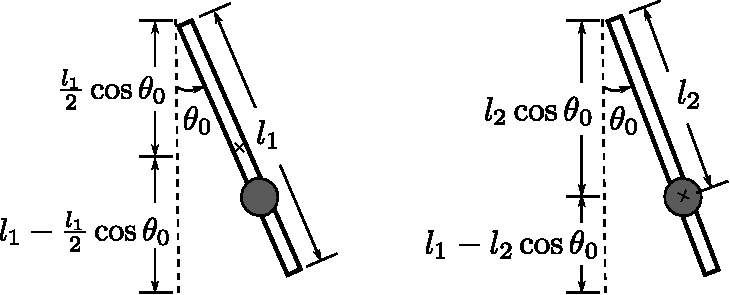
\includegraphics{pendulofisico}
  \caption{Energía potencial inicial del péndulo físico}
  \label{fig:pendulofisico}
\end{figure}

La energía mecánica final es
\begin{align}
  E_f=U_f+K_f=m_1 g \frac{l_1}{2}+m_2 g(l_1-l_2)+\frac{1}{2}I_S \omega_f^2\,.
\end{align}
Igualando las energías inciales y finales
\begin{align}
\label{eq:rig4}
  m_1 g  \left(l_1-\frac{l_1}{2}\cos\theta_0  \right)
+m_2 g  \left(l_1-l_2\cos\theta_0  \right)&=m_1 g \frac{l_1}{2}+m_2 g(l_1-l_2)+\frac{1}{2}I_S \omega_f^2\nonumber\\
  m_1 g  \left(l_1-\frac{l_1}{2}\cos\theta_0  \right)-m_1 g \frac{l_1}{2}-m_2 g(l_1-l_2)
+m_2 g  \left(l_1-l_2\cos\theta_0  \right)&=\frac{1}{2}I_S \omega_f^2\nonumber\\
  m_1 g  \left(l_1-\frac{l_1}{2}\cos\theta_0  \right)-m_1 g \frac{l_1}{2}-\cancel{m_2 g l_1}+\cancel{m_2 gl_1}+m_2 gl_2
-m_2 g  l_2\cos\theta_0 &=\frac{1}{2}I_S \omega_f^2\nonumber\\
  m_1 g  \left(\frac{l_1}{2}-\frac{l_1}{2}\cos\theta_0  \right)+m_2 gl_2
-m_2 g  l_2\cos\theta_0 &=\frac{1}{2}I_S \omega_f^2\nonumber\\
  \frac{m_1 l_1}{2}g \left(1-\cos\theta_0  \right)+
m_2 l_2 g(1-\cos\theta_0) &=\frac{1}{2}I_S \omega_f^2\nonumber\\
  \left(\frac{m_1 l_1}{2}+ m_2 l_2 \right)g \left(1-\cos\theta_0  \right) &=\frac{1}{2}I_S \omega_f^2\,.
\end{align}

Ahora solucionamos para $\omega_f$ (tomando la raíz cuadrada positiva para asegurar que estamos calculando la velocidad angular)
\begin{align}
  \omega_f=\sqrt{\frac{2\left(\frac{m_1 l_1}{2}+ m_2 l_2 \right)g \left(1-\cos\theta_0  \right)}{I_S}}\,.
\end{align}
Finalmente sustituyendo el resultado para $I_S$ de la ec.~\eqref{eq:rig3}
\begin{align}
    \omega_f=\sqrt{\frac{2\left(\frac{m_1 l_1}{2}+ m_2 l_2 \right)g \left(1-\cos\theta_0  \right)}{I_1+I_{\text{cm}}+m_2 l_2^2\,.}}\,.
\end{align}
  \end{enumerate}

Note que podemos reescribir la ec.~\eqref{eq:rig4}, usando la ecuación \eqref{eq:rig5} para la distancia entre el centro de masa y el punto de pivote, y obtener
\begin{align}
\label{eq:rig6}
 (m_1+m_2)l_{\text{cm}} g \left(1-\cos\theta_0  \right) &=\frac{1}{2}I_S \omega_f^2\,. 
\end{align}

Podemos interpretar esta ecuación como sigue. Trate el sistema compuesto como una partícula puntual de masa $m_1+m_2$ localizada en el centro de masa $l_{\text{cm}}$. Tome el punto cero de energía potencial gravitacional para ser el punto donde le centro de masa está en su punto más bajo, esto es, en $\theta=0$. Ver Figura~\ref{fig:pendulofisicocm}. Entonces
\begin{align}
  E_0=(m_1+m_2)l_{\text{cm}} g \left(1-\cos\theta_0  \right)
\end{align}
y
\begin{align}
  E_f=\frac{1}{2}I_S \omega_f^2\,,
\end{align}
de modo que la ecuación \eqref{eq:rig6} se puede obtener directamente de la conservación de la energía del sistema simplificado.
\begin{figure}
  \centering
  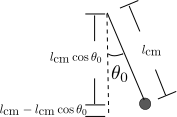
\includegraphics{pendulofisicocm}
  \caption{Sistema visto como un péndulo simple}
  \label{fig:pendulofisicocm}
\end{figure}

\end{itemize}

\begin{itemize}
\item[\textbf{Ejemplo:}] Encuentra la ecuación de movimiento para un péndulo simple de longitud $l$  usando la condición de conservación de la energía mecánica $dE/dt=0$. 

De la Figura.~\ref{fig:pendulofisicocm}, reemplazando $l_{\text{cm}}$ por $l$ y considerando una posición genérica del péndulo formando un ángulo $\theta$ con la vertical podemos calcular la energía mecánica
\begin{align}
 E=& m l g(1-\cos\theta)+\frac{1}{2}I \omega^2\nonumber\\
 =& m l g(1-\cos\theta)+\frac{1}{2}I \dot\theta^2\,.
\end{align}
El momento de inercia para el péndulo simple sobre un eje perpendicular al punto de pivote es
\begin{align}
  I=ml^2\,,
\end{align}
de modo que
\begin{align}
  E=m l g(1-\cos\theta)+\frac{1}{2}m l^2 \dot\theta^2\,.
\end{align}
Aplicando la condición de conservación de la energía mecánica tenemos
\begin{align}
  \frac{dE}{dt}=mlg\dot\theta\sin\theta+\frac{1}{2}m l^2 2\dot\theta\ddot\theta=&0\nonumber\\
mlg\dot\theta\sin\theta+m l^2 \dot\theta\ddot\theta=&0\,.
\end{align}
Simplificando este expresión, tenemos
\begin{align}
 l\ddot\theta+ g\sin\theta=&0\nonumber\\
 \ddot\theta+ \frac{g}{l}\sin\theta=&0\,.
\end{align}
\end{itemize}
Cuando las oscilaciones son pequeñas $\sin\theta\approx\theta$ y
\begin{align}
   \ddot\theta+ \frac{g}{l}\theta=&0\,.
\end{align}
Entonces el péndulo simple realiza un movimiento armónico simple con frecuencia:
\begin{align}
  \omega_0=\sqrt{\frac{g}{l}}
\end{align}
\begin{itemize}
\item[\textbf{Ejemplo:}] Tomado de \cite{mit2009}. Considere una polea de masa $m_p$, radio $R$, y momento de inercia $I_{\text{cm}}$ sobre su centro de masa en uno de los lados de una mesa. Una cuerda inextensible de masa despreciable pasa a través de la polea y esta unida en uno de sus extremos al bloque 1 que cuelga sobre un lado de la mesa. El otro extremo esta unido al bloque 2 que se desliza a lo largo de la mesa. Ver Figura \ref{fig:poleafisica}. El coeficiente de fricción cinético entre la masa y el bloque 2 es $\mu_k$. El bloque 1 tiene una masa $m_1$ y el bloque 2 tiene una masa $m_2$, con $m_1>\mu_k m_2$. En el tiempo $t=0$, los bloques son liberados desde el reposo y la cuerda no se desliza alrededor de la polea,  En el tiempo $t=t_1$, el bloque 1 golpea el piso.
  \begin{enumerate}
  \item Encuentre la magnitud de la aceleración de cada bloque. Exprese su respuesta en términos de $m_p$, $I_{\text{cm}}$, $R$, $m_1$, $m_2$, $\mu_k$, y $t_1$
    \label{item:4}
  \item ¿Cuanto cae el bloque 1 antes de tocar el piso?
    \label{item:5}
  \end{enumerate}

  \begin{figure}
    \centering
    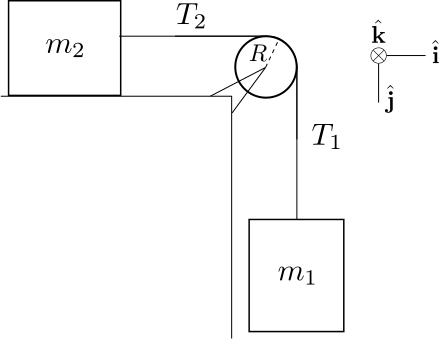
\includegraphics[scale=0.7]{poleafisica}
    \caption{Polea física}
    \label{fig:poleafisica}
  \end{figure}

\ref{item:4}. Escogemos el sistema de referencia tal que los ejes $x$ y $y$ coinciden con el plano de movimiento con $x$ hacia la derecha y $y$ hacia abajo, de modo que  el eje $z$ este entrando a ese plano. 

Entonces, el torque sobre el centro de la polea esta dado por
\begin{align}
  \boldsymbol{\tau}_2+\boldsymbol{\tau}_1=&I_{\text{cm}}\alpha_z\hat{\mathbf{k}}\nonumber\\
  R(-\hat{\mathbf{j}})T_2(-\hat{\mathbf{i}})+R\hat{\mathbf{i}}T_1\hat{\mathbf{j}}=&I_{\text{cm}}\alpha_z\hat{\mathbf{k}}\nonumber\\
  RT_2(-\hat{\mathbf{k}})+RT_1\hat{\mathbf{k}}=&I_{\text{cm}}\alpha_z\hat{\mathbf{k}}\,,
\end{align}
de modo que
%\hat{\mathbf{}}
\begin{align}
  \label{eq:1}
  R(T_1-T_2)=I_{\text{cm}}\alpha_z\,.
\end{align}

La segunda ley de Newton sobre el bloque 1 da lugar a
\begin{align}
  \label{eq:2}
  m_1g-T_1=m_1 a\,.
\end{align}

La segunda ley de Newton sobre el bloque 2 en la dirección $\hat{\mathbf{j}}$, da lugar a
\begin{align}
  N-m_2g=0\,.
\end{align}

La segunda ley de Newton sobre el bloque 2 en la dirección $\hat{\mathbf{i}}$, da lugar a
\begin{align}
  \label{eq:3}
  T_2-f_k=&m_2 a\nonumber\\
  T_2-\mu_k N=&m_2 a\nonumber\\
  T_2-\mu_k m_2 g=&m_2 a\,.
\end{align}

Solucionando las ecs.~\eqref{eq:2} y \eqref{eq:3} para las dos tensiones da lugar a
\begin{align}
  \label{eq:4}
  T_1=&m_1g -m_1 a\nonumber\\
  T_2=&\mu_k m_2 g+m_2 a\,.
\end{align}
El punto en el borde de la polea tiene una aceleración tangencial que es igual a la aceleración de los bloques, de modo que
\begin{align}
  a=R\alpha_z\,.
\end{align}

La ec.~\eqref{eq:1} se puede reescribir como
\begin{align}
  \label{eq:5}
  T_1-T_2=\frac{I_{\text{cm}}}{R^2}a\,.
\end{align}

Sustituyendo la ec.~\eqref{eq:4} en la ec.~\eqref{eq:5} tenemos
\begin{align}
  m_1g -m_1 a-\mu_k m_2 g-m_2 a=\frac{I_{\text{cm}}}{R^2}a\,,
\end{align}
de la cual podemos despejar la aceleración
\begin{align}
    -m_1 a-m_2 a-\frac{I_{\text{cm}}}{R^2}a=&-m_1g+\mu_k m_2 g\nonumber\\
    \left( m_1+m_2+\frac{I_{\text{cm}}}{R^2}\right)a=&m_1g-\mu_k m_2 g\nonumber\\
    a=&\frac{m_1g-\mu_k m_2 g}{m_1+m_2+I_{\text{cm}}/R^2}\,.
\end{align}

\ref{item:5}. El bloque 1 golpea el piso después de un tiempo $t_1$, por consiguiente viajo una distancia
\begin{align}
  y_1=&\frac{1}{2}a t_1^2\nonumber\\
  =&\frac{1}{2}
  \left(
    \frac{m_1g-\mu_k m_2 g}{m_1+m_2+I_{\text{cm}}/R^2}
  \right)t_1^2\,.
\end{align}
\end{itemize}

\begin{itemize}
\item[\textbf{Ejemplo:}] Tomado de \cite{mit2009}: Dos objetos puntuales están localizados en los puntos $A$ y $B$, con masas $m_A=2M$ y $m_B=M$, como se muestra en la figura~\ref{fig:barrabolas} Una fuerza de magnitud $F$ es aplicado a lo largo del eje $x$ al objeto en $B$ de la figura~\ref{fig:barrabolas} en $t=0$ por un intervalo de tiempo $\Delta t$. Despreciando la gravedad, de todas sus respuesta en términos de $M$ y $D$.
  \begin{figure}
    \centering
    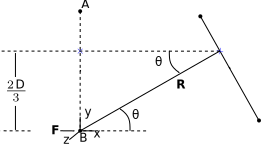
\includegraphics{barrabolas}
    \caption{Sistema de dos partículas de masas diferentes unidos por una barra de masa despreciable.}
    \label{fig:barrabolas}
  \end{figure}

  \begin{enumerate}
  \item Como se mueve el sistema después de aplicar la fuerza.

El sistema rota en el sentido antihorario alrededor del centro de masa, el cual se desplaza a su vez a velocidad constante en la dirección $x$.
\item Cuan lejos esta el centro de masa del sistema desde el punto $B$.

Tomando el origen de coordenadas en el punto medio:
\begin{align}
\mathbf{R}=\frac{m_A(D/2)-m_B(D/2)}{m_A+m_B}\hat{\mathbf{j}}\,.  
\end{align}

\begin{align}
R=&\frac{2M(D/2)-M(D/2)}{3M}\nonumber\\
=&\frac{D-D/2}{3}\nonumber\\
=&\frac{D}{6}\,,
\end{align}
Desde el punto $B$
\begin{align}
  R_B=\frac{D}{2}+\frac{D}{6}=\frac{3D}{6}+\frac{D}{6}=\frac{4D}{6}=\frac{2D}{3}\,.
\end{align}
\item Cual es la magnitud y dirección de la velocidad del centro de masa

  \begin{align}
    \mathbf{F}\cdot \Delta t=\Delta \mathbf{P}=&m_{\text{total}}(\mathbf{V}_{\text{CM}}-\cancel{\mathbf{V}_{\text{CM}}^i})\nonumber\\
    =&(2M+M)\mathbf{V}_{\text{CM}}\nonumber\\
    =&(3M)V_{\text{CM}}\hat{\mathbf{i}}\,.
  \end{align}
de modo que
\begin{align}
  \label{eq:6}
  \mathbf{V}_{\text{CM}}=\frac{F\Delta t}{3M}\,\hat{\mathbf{i}}\,.
\end{align}
\item Cual es la magnitud de la velocidad angular después la colisión:

  \begin{align}
    \label{eq:7}
    \mathbf{L}_f=&\mathbf{R}\timesm M\mathbf{V}_{CM}+\mathbf{L}_0\,,
  \end{align}
donde $\mathbf{L}_f$ es el momento angular final. Como el correspondiente momento angular inicial es cero
\begin{align}
    \mathbf{L}_i=&\mathbf{R}\timesm \mathbf{V}_{CM}^i\,,
\end{align}
pues la velocidad inicial del centro de masa es cero, y como el correspondiente torque en el punto $B$ durante la  aplicación de la fuerza es cero:
\begin{align}
  \boldsymbol{\tau}_B=\mathbf{0}\timesm \mathbf{F}=0\,. 
\end{align}
Por consiguiente el momento angular alrededor del punto $B$ se conserva y
\begin{align}
  \mathbf{L}_f=\mathbf{L}_i=0\,,
\end{align}
y reemplazando en la ec.~(\ref{eq:7}), tenemos
\begin{align}
  \mathbf{L}_0=& -\mathbf{R}\timesm M\mathbf{V}_{CM}\nonumber\\
=& -\mathbf{R}\timesm \mathbf{P}\nonumber\\
=& -\mathbf{R}\timesm \mathbf{P}-\mathbf{P}_i\nonumber\\
=& -\mathbf{R}\timesm \Delta \mathbf{P}\nonumber\\
=& -\mathbf{R}\timesm \mathbf{F}\Delta t\nonumber\\
\end{align}
Para interpretar correctamente es producto vectorial $\mathbf{R}\timesm \mathbf{F}$ considere el diagrama en la fig.~\ref{fig:barrabolas2}, donde $\mathbf{R}$ es el que une el origen de coordenadas con el centro de masa. El ángulo entre los vectores $\mathbf{R}$ y $\mathbf{F}$ es $\theta$, de modo que
\begin{align}
  \mathbf{L}_0=&-(R \sin\theta)F \Delta t(-\hat{\mathbf{k}})\nonumber\\
=&(R \sin\theta)F \Delta t\,\hat{\mathbf{k}}\,.
\end{align}


\begin{figure}
  \centering
  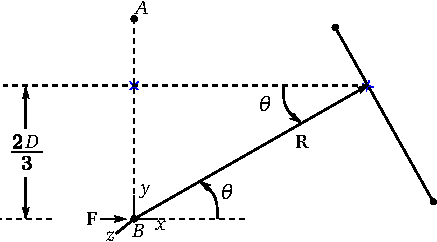
\includegraphics{barrabolas2}
  \caption{Producto vectorial $\mathbf{R}\timesm \mathbf{F}$}
  \label{fig:barrabolas2}
\end{figure}

De la fig.~\ref{fig:barrabolas2} también tenemos que
\begin{align}
  R\sin\theta=\frac{2D}{3}\,,
\end{align}
de modo que
\begin{align}
\label{eq:8}
\mathbf{L}_0= \frac{2D}{3} F\Delta t\,\hat{\mathbf{k}}\,.
\end{align}

De otro lado el momento angular alrededor del centro de masa satisface la ecuación de movimiento
\begin{align}
  \label{eq:9}
  \mathbf{L}_0=I_{\text{CM}}\omega\,\hat{\mathbf{k}}\,,
\end{align}
donde, el momento de inercia sobre el centro de masa esta dados por las distancias desde el centro de masa a cada una de las partículas:
\begin{align}
  \label{eq:10}
  I_{\text{CM}}=&m_A {r'_{A}}^2+m_B {r'_{B}}^2\nonumber\\
  =&2M \left(\frac{D}{3}\right)^2+M\left(\frac{2D}{3}\right)^2\nonumber\\
  =&M D^2 \left(\frac{2}{9}+\frac{4}{9}\right)\nonumber\\
   =&\frac{6}{9}M D^2 \nonumber\\
   =&\frac{2D}{3}M D\,.
\end{align}

Reemplazando las ecs.~\eqref{eq:8} y \eqref{eq:10} en \eqref{eq:9}, obtenemos
\begin{align}
  \frac{2D}{3} F\Delta t=\frac{2D}{3}M D \omega\,,
\end{align}
y despejando para la velocidad angular, obtenemos el resultado final
\begin{align}
  \omega=\frac{F\Delta t}{M D}\,.
\end{align}

%\left(\right)
  \end{enumerate}

  \begin{itemize}
  \item Hallar la aceleración de un cilindro uniforme de radio $R$ y masa $M$ cuando rueda sin deslizar por un plano inclinado a un ángulo $\beta$
  \end{itemize}
  \begin{itemize}
  \item Aplicando la ecuación de torque sobre el centro de masa:...

  \end{itemize}

  \begin{itemize}
  \item[\textbf{Ejemplo:}] Ejemplo 27.7.4 (pag. 17) de \cite{mit2009}: \textbf{Cilindro rodando hacia abajo de un plano inclinado}.
  \end{itemize}
\end{itemize}

\section{Ecuaciones de Euler}


Suponga un sistema rotando a través de sus tres ejes principales, de modo que las componentes de $\mathbf{L}$ son
\begin{align}
  \mathbf{L}=(I_1\omega_1,I_2\omega_2,I_3\omega_3)
\end{align}

Hay dos formas en las cuales $L_1$ puede cambiar: por cambios en $\omega_1$, o cambios en $L_2$ y $L_3$. Fijemos las posible rotaciones a lo largo de los ejes en el sentido de la mano derecha. Entonces
\begin{align}
  \label{eq:DL1}
  \Delta L_1=I_1\Delta\omega_1+\Delta(L_2)+\Delta(L_3)\,,
\end{align}
consideremos primero la rotación sobre el eje principal 2. Esta induce un cambio en el moméntum angular $L_1$ que contribuye a la ec.~\eqref{eq:DL1} como
\begin{align}
    \Delta L_1=&I_1\Delta\omega_1+L_3\sin(\Delta\theta_2)+\Delta(L_3)\nonumber\\
    =&I_1\Delta\omega_1+I_3\omega_3\Delta\theta_2+\Delta(L_3)\,.
\end{align}
Similarmente, una rotación sobre el eje principal 3
\begin{align}
    \Delta L_1=&I_1\Delta\omega_1+I_3\omega_3\Delta\theta_2-I_2\omega_2\Delta\theta_3\,.
\end{align}
\begin{align}
  \lim_{\Delta t\to 0}\frac{\Delta L_1}{\Delta t}=&
I_1\frac{d\omega_1}{dt}+(I_3-I_2)\omega_2\omega_3\,.
\end{align}
Repitiendo el mismo proceso para $L_2$ y $L_3$ obtenemos las ecuaciones de Euler para el movimiento del cuerpo rígido
\begin{align}
  \tau_1=\frac{dL_1}{dt}=&I_1\frac{d\omega_1}{dt}+(I_3-I_2)\omega_2\omega_3\nonumber\\
  \tau_2=\frac{dL_2}{dt}=&I_2\frac{d\omega_2}{dt}+(I_1-I_3)\omega_1\omega_3\nonumber\\
  \tau_3=\frac{dL_3}{dt}=&I_3\frac{d\omega_3}{dt}+(I_2-I_1)\omega_2\omega_1\,.
\end{align}
\subsection{Estabilidad del movimiento rotacional}
\begin{align}
\omega_1=&\text{cte}&   \omega_2=&0& \omega_3=&0\,,
\end{align}
después de una pequeña perturbación
\begin{align}
  \omega_2\ne&0\,,&\omega_3\ne&0\,,\qquad\text{pero}\nonumber\\
  \omega_2\ll& \omega_1 \,,&\omega_3\ll &\omega_1\,.
\end{align}

se llega a las ecuaciones
\begin{align}
  \frac{d\omega_1}{dt}=&0\nonumber\\
  \frac{d^2\omega_2}{dt^2}+A\omega_2=&0\,,
\end{align}
donde
\begin{align}
  A=\frac{(I_1-I_2)(I_1-I_3)}{I_2I_3}\omega_1^2\,.
\end{align}
Si $A>0$ tenemos una solución oscilatoria, que corresponde a un movimiento de precesión a lo largo del eje 1, el cual es un movimiento de rotacional estable. Si $A>0$, la solución es
\begin{align}
  \omega_2 C\exp(A^2 t)
\end{align}
(donde $C$ es una constante por especificar) de modo que $w_2$ se incrementa exponencialmente con el tiempo, dando lugar a un movimiento inestable.

El movimiento estable, es decir con $A>0$, cuando $I_1=I_{\text{max}}$ ó si  $I_1=I_{\text{min}}$. El movimiento es inestable, es decir con $A<0$, cuando $I_1$ es el momento de inercia intermedio.

\begin{itemize}
\item[\textbf{Ejemplo:}] Tomado de \cite{mit2009}: Un disco con momento de inercia sobre el centro de masa $I_{\text{cm}}$ rota en un plano horizontal. Está suspendido por una varilla delgada de masa despreciable. Si el disco se rota fuera de su posición de equilibrio por un ángulo $\theta$, la varilla ejerce una torque restaurardor dado por $\boldsymbol{\tau}_{\text{cm}}=-\gamma \theta$. En $t=0$ el disco es liberado desde el reposo con un desplazamiento angular de $\theta_0$. Encuentre la subsecuente dependencia temporal del desplazamiento angular $\theta(t)$


Escojamos un sistema de coordenadas tal que $\hat{\mathbf{k}}$ apunte hacia arriba.  La componente $\hat{\mathbf{k}}$ de la ecuación de torque
\begin{align}
  \boldsymbol{\tau}_{\text{cm}}=I_{\text{cm}}\boldsymbol{\alpha}\,,
\end{align}
es
\begin{align}
  -\gamma \theta= I_{\text{cm}}\frac{d^2\theta}{d t^2}\,.
\end{align}
o
\begin{align}
\frac{d^2\theta}{d t^2}+\frac{\gamma}{I_{\text{cm}}}\theta=0\,.
\end{align}

Esto es una ecuación de un oscilador armónico simple con solución
\begin{align}
  \theta(t)=A\cos(\omega_0 t)+B\sin(\omega_0 t)\,.
\end{align}
Donde la frecuencia de oscilación está dada por
\begin{align}
  \omega_0=\sqrt{\gamma/I_{\text{cm}}}\,.
\end{align}
La componente $z$ de la velocidad angular está dada por
\begin{align}
  \frac{d\theta(t)}{dt}=-A\omega_0\sin(\omega_0 t)+B\omega_0\sin(\omega_0 t)\,.
\end{align}

Las condiciones iniciales en $t=0$, son que $\theta(t=0)=A=\theta_0$, y $d\theta/dt=0=\omega_0B$, de donde $B=0$. Entonces
\begin{align}
   \theta(t)=\theta_0\cos\left(\sqrt{\gamma/I_{\text{cm}}} t \right)\,.
\end{align}
\end{itemize}

\section{Problemas resueltos}

\begin{enumerate}
\item (Tomado de \cite{gabriel}) Un bloque de masa $m$ desliza por la superficie del plano inclinado de ángulo $\theta$, mostrado en la figura. El coeficiente de fricción entre el bloque y la superficie es $\mu$. Por la acción de la cuerda, el cilindro macizo de masa $M$ y radio $R$ gira alrededor de un eje fijo que para por $C$.  La cuerda esta enrollada alrededor de un pequeño saliente de radio $r=0.1\ $m. Desprecie la fricción entre el volante y el eje alrededor del cual gira. 

  \begin{minipage}{0.3\linewidth}
    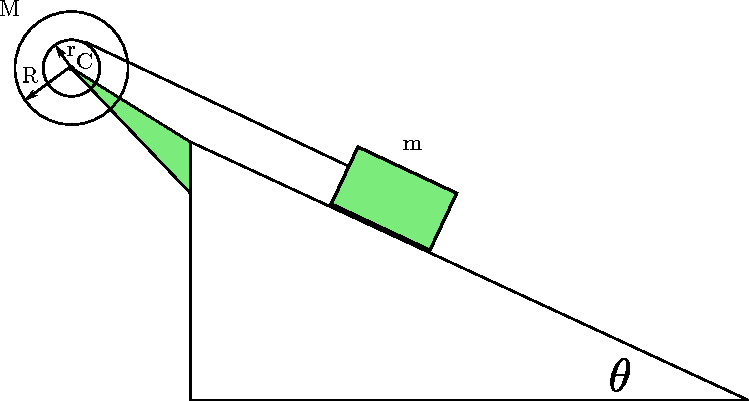
\includegraphics[scale=0.45]{poleasuple}
  \end{minipage}
  \begin{minipage}{0.7\linewidth}
    \begin{enumerate}
    \item Haga el diagrama de fuerzas que actúan sobre cada uno de los cuerpos.
      \label{item:p3a}
    \item Escriba las ecuaciones de movimiento para estos cuerpos.
      \label{item:p3b}
    \item Encuentre la tensión en la cuerda, la aceleración angular del volante y la aceleración del bloque. 
      \label{item:p3c}
    \item Hallar la energía cinética rotacional del sistema cuando el bloque ha recorrido una distancia $h$. 
    \item Finalmente, calcule las cantidades anteriores para el caso particular de $m=5\ $Kg, $\mu=0.25$, $M=20\ $Kg, $R=0.2\ $m $r=0.1\ $m, $\theta=37^\circ$
    \end{enumerate}
  \end{minipage}
%sln pag 183

  \begin{itemize}
  \item[\textbf{Solución}]
  \item[\ref{item:p3b}] 
    Para la polea, si el eje $z$ apunta hacia afuera de la página:
    \begin{align*}
      \boldsymbol{\tau}=&I\boldsymbol{\alpha}\nonumber\\
      -rT=&-I_c\alpha\,.
    \end{align*}
    Para el bloque
    \begin{align*}
      mg\sin\theta-T-\mu N=&m a\nonumber\\
      N=&mg\cos\theta\,.
    \end{align*}
  \item[\ref{item:p3c}]
    Usando la ligadura
    \begin{align*}
      a=&r\alpha\,,
    \end{align*}
    Tenemos
    \begin{align*}
      T=\frac{I_c}{r^2}a
    \end{align*}
    y sustityendo en la ecuación de movimiento para el bloque
    \begin{align*}
      mg\sin\theta-\frac{I_c}{r^2}a-\mu g \cos\theta=&ma\,,
    \end{align*}
    podemos despejar $a$
    \begin{align*}
      a(m+I_c/r^2)=&mg(\sin\theta-\mu\cos\theta)\nonumber\\
      a=&\frac{mg(\sin\theta-\mu\cos\theta)}{m+I_c/r^2}\nonumber\\
      =&\frac{mg(\sin\theta-\mu\cos\theta)}{m+MR^2/(2r^2)}\nonumber\\
      =&\frac{2r^2mg(\sin\theta-\mu\cos\theta)}{2r^2m+MR^2}\,,
    \end{align*}
    y reemplzando de nuevo en $T$
    \begin{align*}
      T=\frac{MR^2}{2r^2}a\,.
    \end{align*}

  \end{itemize}

\item Un cilíndro de radio $R$ y masa $M$ rueda sin deslizar a lo largo
    de una superficie debido a una cinta delgada enrollada en torno de
    el, que pasa por una polea ideal y está conectada a un bloque de
    masa $m$ como se muestra en la figura.


\begin{minipage}{9 cm}

\includegraphics[scale=0.8]{cilindropol}

\end{minipage}
\begin{minipage}{8 cm}
\begin{enumerate}
\item Haga un diagrama de cuerpo libre para cada cuerpo.
      \label{item:r3a}
\item Plantee las ecuaciones de movimiento para cada cuerpo.
      \label{item:r3b}
\item Halle la aceleración del cilindro y la aceleración del bloque
      \label{item:r3c}
\item Calcule la tensión en la cuerda para $M=1$ kg, $m=750$ g
      \label{item:r3d}
\end{enumerate}
\end{minipage}
%variaciones: plano inclinado pag 181,  y polea no ideal, pag. 185

\begin{itemize}
\item[\ref{item:r3b}] Para el cilíndro y tomando los torques con respecto al punto de contacto con la superficie
  \begin{align*}
    -T-f=&M a_{\text{CM}}\\
    N=&Mg\\
    2 R T=I_p \alpha\,,
  \end{align*}
Para el cuerpo
\begin{align*}
  T-m g=&-ma\,.
\end{align*}
\item[\ref{item:r3c}] La aceleración del cilindro $a_{\text{CM}}$, la aceleración angular $\alpha$, y la aceleración $a$ del bloque están relacionadas por
  \begin{align*}
    a=2\alpha R=2 a_{\text{CM}}
  \end{align*}
Entonces, de la ecuación de movimiento para el cilindro
\begin{align*}
  a_{\text{CM}}=&\alpha R\\
  =&\frac{2 R^2 T}{I_p}\\
  =&\frac{2 R^2 T}{\frac{3}{2}MR^2}\\
  =&\frac{4 T}{3M}\,
\end{align*}
y para el cuerpo
\begin{align*}
  a=&\frac{mg-T}{m}\\
  a_{\text{CM}}=\frac{a}{2}=&\frac{mg-T}{2m}\\
  =&\frac{g}{2}-\frac{T}{2m}\,.
\end{align*}
Igualanado las expresiones podemos obtener la tensión
\begin{align*}
\frac{4 T}{3M}=&\frac{g}{2}-\frac{T}{2m}\\
  \frac{4 T}{3M}+\frac{T}{2m}=&\frac{g}{2}\\
  T  \left(\frac{4 }{3M}+\frac{1}{2m}\right)=&\frac{g}{2}\\
  T  \left(\frac{8m+3M }{6Mm}\right)=&\frac{g}{2}\\
  T=&\frac{3Mmg}{8m+3M}\,,
\end{align*}
finalmente, reemplazando en la primera expresión para $a_{\text{CM}}$
\begin{align*}
  a_{\text{CM}}=&\frac{4}{3M}\frac{3Mmg}{8m+3M}\\
=&\frac{4mg}{8m+3M}\,.
\end{align*}


Por conservación de la energía...

\end{itemize}
\end{enumerate}

%%% Local Variables: 
%%% mode: latex
%%% TeX-master: "mecanica"
%%% End: 
